% Standalone supplementary material for the restructured manuscript.
% Compile after paper/main.tex so build/main.aux is available for cross-references.
\documentclass[10pt]{article}
\usepackage[utf8]{inputenc}
\usepackage{tmlr}
\usepackage{amsmath,amssymb}
\usepackage{graphicx}
\usepackage{pdflscape}
\usepackage{longtable,booktabs,array,calc}
\usepackage{url}
\usepackage[hidelinks]{hyperref}
\usepackage{bookmark}
\usepackage[nameinlink,noabbrev]{cleveref}
\usepackage{xurl}
\usepackage{xr-hyper}
\externaldocument{build/main}
\bibliographystyle{tmlr}

\title{Supplementary Material: Activation-Patching Effects in Controlled CNNs}
\author{}
\date{}

\begin{document}
\maketitle

This supplement preserves the exhaustive numerical record without requiring the main paper to carry every table. It is organized by evidential role rather than by the chronology in which the experiments were conducted. The main manuscript contains the comparisons needed to understand and evaluate the central conclusions; the material below provides implementation checks, complete estimates, sensitivity analyses, and the earlier exploratory record.

\section*{Supplementary Block I: Methods and checks}

This block contains structural matching checks and implementation-level diagnostics used to verify that the reported intervention quantities correspond to the intended first-layer filters and checkpoints.

\begin{figure}[t]
\centering
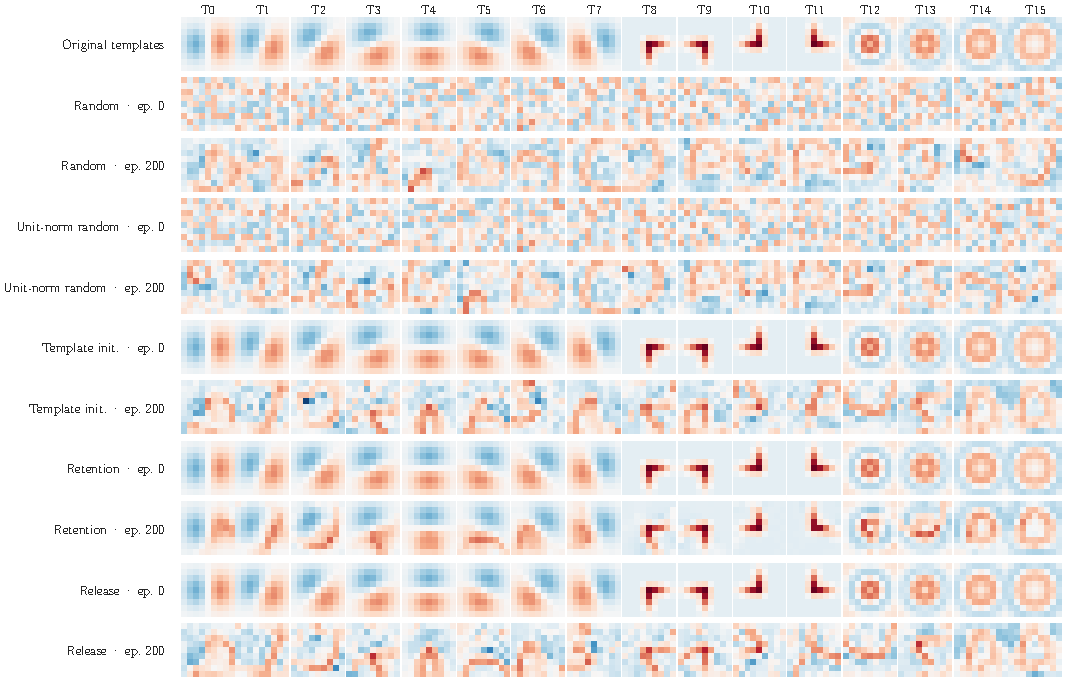
\includegraphics[width=\linewidth]{figures/fig05_kernel_gallery.pdf}
\caption{Complete 16-channel kernel gallery retained as a supplementary structural diagnostic. The main manuscript uses only the compact checkpoint-based subset.}
\label{fig:supp-full-kernels}
\end{figure}

\section{Complete filter-matching table}\label{app:kernel-matching}

The main Results section contains three visual summaries of this exploratory Stage-B follow-up: the matching trajectories, the complete similarity matrices for one replicate, and the matched filter gallery. This appendix therefore reports only the complete epoch-200 numerical table.

All values below are epoch-200 means $\pm$ sample standard deviation across ten replicates; conditions are paired within replicate. The nearest-template and one-to-one scores use signed cosine similarity. Coverage counts distinct nearest-template entries; because the bank has rank 10, it is neither a count of linearly independent directions nor a count of independent semantic concepts. The analysis uses only saved Stage-B checkpoints. These descriptive comparisons are exploratory.

{\footnotesize
\setlength{\tabcolsep}{2.5pt}
\begin{longtable}{p{.15\linewidth}p{.17\linewidth}p{.20\linewidth}rrr}
\caption{Epoch-200 filter-template matching results.}\label{tab:kernel-matching-full}\\
\toprule
Task & Architecture & Condition & Nearest-template & One-to-one & Coverage \\
\midrule
\endfirsthead
\toprule
Task & Architecture & Condition & Nearest-template & One-to-one & Coverage \\
\midrule
\endhead
\bottomrule
\endfoot
single shape & TinyCNN & random & 0.300 $\pm$ 0.023 & 0.267 $\pm$ 0.033 & 9.700 $\pm$ 1.703 \\
single shape & TinyCNN & unit-norm random & 0.288 $\pm$ 0.022 & 0.256 $\pm$ 0.034 & 9.700 $\pm$ 1.703 \\
single shape & TinyCNN & initialization only & 0.610 $\pm$ 0.021 & 0.605 $\pm$ 0.021 & 13.300 $\pm$ 1.337 \\
single shape & TinyCNN & annealed regularization & 0.690 $\pm$ 0.017 & 0.686 $\pm$ 0.017 & 14.200 $\pm$ 1.033 \\
single shape & TinyCNN & constant $\lambda=1$ regularization & 0.959 $\pm$ 0.003 & 0.959 $\pm$ 0.003 & 16.000 $\pm$ 0.000 \\
\addlinespace[2pt]
single shape & TwoLayerCNN & random & 0.261 $\pm$ 0.037 & 0.230 $\pm$ 0.039 & 9.200 $\pm$ 1.317 \\
single shape & TwoLayerCNN & unit-norm random & 0.228 $\pm$ 0.033 & 0.195 $\pm$ 0.039 & 8.300 $\pm$ 1.889 \\
single shape & TwoLayerCNN & initialization only & 0.799 $\pm$ 0.015 & 0.799 $\pm$ 0.015 & 15.700 $\pm$ 0.483 \\
single shape & TwoLayerCNN & annealed regularization & 0.942 $\pm$ 0.006 & 0.942 $\pm$ 0.006 & 16.000 $\pm$ 0.000 \\
single shape & TwoLayerCNN & constant $\lambda=1$ regularization & 1.000 $\pm$ 0.000 & 1.000 $\pm$ 0.000 & 16.000 $\pm$ 0.000 \\
\addlinespace[2pt]
two concepts & TinyCNN & random & 0.232 $\pm$ 0.034 & 0.199 $\pm$ 0.035 & 9.100 $\pm$ 1.524 \\
two concepts & TinyCNN & unit-norm random & 0.222 $\pm$ 0.031 & 0.191 $\pm$ 0.037 & 9.200 $\pm$ 1.398 \\
two concepts & TinyCNN & initialization only & 0.507 $\pm$ 0.022 & 0.496 $\pm$ 0.022 & 12.000 $\pm$ 1.054 \\
two concepts & TinyCNN & annealed regularization & 0.580 $\pm$ 0.011 & 0.574 $\pm$ 0.010 & 12.900 $\pm$ 0.994 \\
two concepts & TinyCNN & constant $\lambda=1$ regularization & 0.947 $\pm$ 0.004 & 0.947 $\pm$ 0.004 & 16.000 $\pm$ 0.000 \\
\addlinespace[2pt]
two concepts & TwoLayerCNN & random & 0.255 $\pm$ 0.027 & 0.231 $\pm$ 0.024 & 9.600 $\pm$ 1.075 \\
two concepts & TwoLayerCNN & unit-norm random & 0.243 $\pm$ 0.028 & 0.218 $\pm$ 0.027 & 9.000 $\pm$ 1.054 \\
two concepts & TwoLayerCNN & initialization only & 0.746 $\pm$ 0.017 & 0.746 $\pm$ 0.017 & 15.400 $\pm$ 0.699 \\
two concepts & TwoLayerCNN & annealed regularization & 0.907 $\pm$ 0.012 & 0.907 $\pm$ 0.012 & 16.000 $\pm$ 0.000 \\
two concepts & TwoLayerCNN & constant $\lambda=1$ regularization & 0.999 $\pm$ 0.000 & 0.999 $\pm$ 0.000 & 16.000 $\pm$ 0.000 \\
\end{longtable}
\normalsize
}

\section*{Supplementary Block II: Complete estimates and sensitivity analyses}

This block contains the full spatial-control, metric-sensitivity, architecture-robustness, intervention-size, schedule/task, channel-selection, and numerical-audit results. These tables provide the exhaustive estimates behind the compact figures and summaries in the main paper.

\section{Pixel-permuted control and architecture analyses}\label{app:specificity}

This appendix reports the complete numerical results for the pixel-permuted control experiment and the post-hoc architecture analyses. The control experiment was specified before evaluation on independent renderer blocks; the architecture analyses were performed post-hoc after the original architecture results were known and are labeled accordingly.

\subsection{Pixel-permuted control experiment}\label{app:anchor-specificity}

The experiment uses 100 independent renderer blocks, four initialization/filter-bank replicates per block, two tasks, four architectures, four filter-bank families, and two regularization schedules, for 25,600 trained and evaluated models. The independent unit for inference is the renderer block after averaging the four within-block replicates.

The primary comparison is the original structured edge/corner/ring bank against a bank formed by applying one common random permutation of the 81 spatial coordinates to every template row. This pixel-permuted control preserves, to numerical tolerance, every row norm, the complete $16\times16$ Gram matrix, numerical rank, singular spectrum, and row coefficient multisets while destroying the original 2D spatial arrangement.

\begin{table}[h]
\caption{Structured-minus-pixel-permuted difference in the selected-channel $B$ contrast, averaged across architectures on \texttt{two\_concepts}. Difference tests use 100,000 sign-flip permutations and Holm correction across the two output metrics. Equivalence uses the pre-specified TOST margins and 90\% confidence intervals.}
\label{tab:anchor-primary}
\centering
\footnotesize
\setlength{\tabcolsep}{3pt}
\begin{tabular}{lrrrr}
\toprule
Metric & Mean difference & 95\% CI & Holm diff. $p$ & Equivalence result \\
\midrule
Centered-logit fidelity & +0.05743 & [0.05116, 0.06369] & $2.0\times10^{-5}$ & not equivalent ($\delta=0.01704$) \\
Probability error reduction & +0.04563 & [0.03728, 0.05397] & $2.0\times10^{-5}$ & equivalent ($\delta=0.06594$) \\
\bottomrule
\end{tabular}
\end{table}

The equivalence margins were pre-specified before the new outcomes as 20\% of the mean absolute $B$ from the earlier architecture study for the same four architectures: $\delta_{\mathrm{clogit}}=0.01704$ and $\delta_{R_{\mathrm{prob}}}=0.06594$. These are study-specific equivalence margins rather than externally validated thresholds of scientific importance. For centered logits, the 90\% interval averaged across architectures is $[0.05219,0.06266]$ and the Holm-adjusted TOST $p$ value is 1. For probability error reduction, the 90\% interval averaged across architectures is $[0.03864,0.05261]$ and the Holm-adjusted TOST $p$ value is $5.03\times10^{-6}$. Thus the probability-error difference averaged across architectures is statistically nonzero while falling inside the pre-specified equivalence region. The smallest symmetric margin that would contain its observed 90\% interval is approximately $0.05261$, about 16.0\% of the effect scale from the earlier architecture study used to define the pre-specified 20\% margin; this sensitivity is reported to make the role of the margin explicit.

\subsection{Architecture dependence of the spatial-arrangement effect}\label{app:anchor-architecture}

The structured-minus-pixel-permuted effect varies strongly across the four pre-specified architectures.

\begin{table}[h]
\caption{Architecture-specific selected-channel structured-minus-pixel-permuted $B$ differences on \texttt{two\_concepts}. Intervals are paired 95\% $t$ intervals over 100 renderer blocks.}
\label{tab:anchor-architectures}
\centering
\small
\begin{tabular}{lrr}
\toprule
Architecture & Centered-logit difference & Probability-error difference \\
\midrule
\texttt{tiny\_gmp} & +0.10624 & +0.19953 \\
\texttt{tiny\_gap} & +0.07690 & +0.04308 \\
\texttt{plain2\_w16\_gmp} & -0.04453 & -0.08067 \\
\texttt{plain2\_w16\_gap} & +0.09109 & +0.02057 \\
\bottomrule
\end{tabular}
\end{table}

The corresponding within-block architecture interaction is
$F(3,297)=91.79$, partial $\eta^2=0.481$, Holm permutation $p=2.0\times10^{-5}$ for centered-logit fidelity, and
$F(3,297)=157.70$, partial $\eta^2=0.614$, Holm permutation $p=2.0\times10^{-5}$ for probability error reduction. The sign reversal in \texttt{plain2\_w16\_gmp} rules out a universal positive effect of the original spatial arrangement.

\subsection{Random-channel control}\label{app:anchor-random}

Repeating the primary comparison after averaging over eight random channel orders produces much smaller effects of the original spatial arrangement.

\begin{table}[h]
\caption{Structured-minus-pixel-permuted $B$ averaged across architectures for random channel sets on \texttt{two\_concepts}. Both effects are statistically distinguishable from zero and fall within the pre-specified equivalence margins.}
\label{tab:anchor-random}
\centering
\small
\begin{tabular}{lrr}
\toprule
Metric & Mean difference & 95\% CI \\
\midrule
Centered-logit fidelity & +0.00571 & [0.00392, 0.00750] \\
Probability error reduction & +0.02007 & [0.01722, 0.02291] \\
\bottomrule
\end{tabular}
\end{table}

The interaction between filter-bank type and architecture for random channels remains detectable but is smaller for centered logits: partial $\eta^2=0.0683$ with permutation $p=8.0\times10^{-5}$. For probability error reduction it remains substantial, partial $\eta^2=0.2910$ with permutation $p=1.0\times10^{-5}$. Thus small random-channel effects averaged across architectures coexist with architecture-dependent differences; the equivalence statements apply to the averages across architectures, not to every architecture separately. These are pre-specified secondary analyses.

Secondary filter-bank contrasts show that the pixel-permuted and generic random rank-10 banks are generally similar on the primary task, and that the random rank-10 and random full-rank banks are also generally similar after the pre-specified Holm corrections. The original 2D arrangement, rather than numerical rank alone, is therefore the filter-bank property most clearly distinguished by the selected-channel analysis.

The full-patch and no-op checks give zero logit error, as required. The maximum structured-versus-pixel-permuted Gram-matrix discrepancy is $6.66\times10^{-16}$.

\subsection{Post-hoc architecture analyses}\label{app:architecture-posthoc}

\paragraph{Exact architecture definitions.}
All variants share the same patched $1\!\to\!16$, $9\times9$ first convolution and ReLU. Pooling is global max (GMP) or global average (GAP). Plain depth-2 networks add one $3\times3$ convolution; plain depth-4 networks add three. Width-64 variants expand the first downstream convolution to 64 channels and remain width 64 thereafter. Residual depth-4 variants keep width 16 and add the third downstream convolution to the original first-layer activation before the final ReLU. BatchNorm, when present, is downstream of the intervention tensor.

\begin{table}[h]
\caption{Exact architecture grid used in the pre-specified architecture study. Parameter counts include the classifier.}
\label{tab:architecture-definitions}
\centering
\scriptsize
\setlength{\tabcolsep}{3pt}
\begin{tabular}{lrrrrlr}
\toprule
Architecture & Conv depth & Width & Pool & BN & Connectivity & Parameters \\
\midrule
\texttt{tiny\_gmp} & 1 & 16 & GMP & no & none & 1,364 \\
\texttt{tiny\_gap} & 1 & 16 & GAP & no & none & 1,364 \\
\texttt{plain2\_w16\_gmp} & 2 & 16 & GMP & no & plain & 3,684 \\
\texttt{plain2\_w16\_gap} & 2 & 16 & GAP & no & plain & 3,684 \\
\texttt{plain4\_w16\_gmp} & 4 & 16 & GMP & no & plain & 8,324 \\
\texttt{plain4\_w16\_gap} & 4 & 16 & GAP & no & plain & 8,324 \\
\texttt{plain2\_w64\_gmp} & 2 & 64 & GMP & no & plain & 10,836 \\
\texttt{plain2\_w64\_gap} & 2 & 64 & GAP & no & plain & 10,836 \\
\texttt{plain4\_w64\_gmp} & 4 & 64 & GMP & no & plain & 84,692 \\
\texttt{plain4\_w64\_gap} & 4 & 64 & GAP & no & plain & 84,692 \\
\texttt{res4\_w16\_gmp} & 4 & 16 & GMP & no & residual & 8,324 \\
\texttt{res4\_w16\_gap} & 4 & 16 & GAP & no & residual & 8,324 \\
\texttt{bn2\_w16\_gmp} & 2 & 16 & GMP & yes & plain & 3,700 \\
\texttt{bn2\_w16\_gap} & 2 & 16 & GAP & yes & plain & 3,700 \\
\texttt{bn4\_w16\_gmp} & 4 & 16 & GMP & yes & plain & 8,372 \\
\texttt{bn4\_w16\_gap} & 4 & 16 & GAP & yes & plain & 8,372 \\
\bottomrule
\end{tabular}
\end{table}

The original 16-architecture study was pre-specified. After seeing its results, separate post-hoc analyses tested whether the omnibus conclusion depended on the uncorrected sphericity assumption or on the validation-based channel ranking.

\begin{table}[h]
\caption{Sphericity-corrected and permutation-based architecture omnibus analyses on the primary \texttt{two\_concepts} task. Permutation $p$ values use 100,000 within-block permutations and are Holm adjusted across the two metrics within each analysis kind.}
\label{tab:architecture-posthoc}
\centering
\footnotesize
\setlength{\tabcolsep}{3pt}
\begin{tabular}{lrrrr}
\toprule
Metric & GG $\epsilon$ & GG $p$ & Permutation Holm $p$ & Friedman $p$ \\
\midrule
Centered-logit fidelity & 0.1861 & $1.56\times10^{-34}$ & $2.0\times10^{-5}$ & $3.52\times10^{-146}$ \\
Probability error reduction & 0.5973 & $<10^{-300}$ & $2.0\times10^{-5}$ & $7.79\times10^{-200}$ \\
\bottomrule
\end{tabular}
\end{table}

Differences across architectures also remain when $B$ is computed from the mean over eight random channel orders: Holm-adjusted permutation $p=2.0\times10^{-5}$ for both output metrics. The Spearman correlation across architecture means for selected versus random channels is $0.256$ for centered logits and $0.724$ for probability error reduction.

For the TinyGMP-minus-Plain2-GMP contrast using random channel sets, the mean difference is $+0.002765$ (95\% CI $[+0.000014,+0.005515]$, Holm $p=0.0488$) for centered logits and $+0.319871$ (95\% CI $[+0.312788,+0.326953]$, Holm $p=2.76\times10^{-96}$) for probability error reduction. The architecture conclusion is therefore not solely a consequence of the selected-channel ranking, although the ranking changes effect magnitude and the ordering across architectures.

\clearpage
\section{Metric sensitivity and architecture results}\label{app:final-robustness}

This appendix gives the complete numerical results for the pre-specified metric-sensitivity reanalysis and the pre-specified architecture study. Block-level values, supporting tables, and control analyses are versioned under \texttt{analysis/metric\_sensitivity\_001/} and \texttt{analysis/architecture\_robustness\_001/}. The main text reports the principal estimates.

\subsection{Metric-sensitivity analysis}\label{app:metric-sensitivity}

The metric-sensitivity analysis reuses saved checkpoints from the pre-specified intervention-size and schedule/task sensitivity experiments. It was designed after the original probability-fidelity results were known, so it is post-hoc with respect to those results; however, the alternative metric definitions and analysis plan were specified before their values were computed. No model was retrained and the original validation-derived channel rankings were reused.

For the primary \texttt{two\_concepts}/TinyCNN setting, \Cref{tab:app-metric-pointwise} gives the full pointwise annealed-minus-constant curves under the two alternative evaluation metrics.

\begin{table}[h]
\caption{TinyCNN pointwise release-minus-retention contrasts under the pre-specified alternative metrics.}
\label{tab:app-metric-pointwise}
\centering
\small
\begin{tabular}{lrrr}
\toprule
Metric & $k$ & Mean $\Delta$ & 95\% CI \\
\midrule
Centered-logit fidelity & 1 & -0.21134 & [-0.27899, -0.14369] \\
Centered-logit fidelity & 2 & -0.17452 & [-0.22078, -0.12825] \\
Centered-logit fidelity & 4 & -0.03405 & [-0.04939, -0.01871] \\
Centered-logit fidelity & 8 & +0.00595 & [+0.00253, +0.00937] \\
\addlinespace[2pt]
Probability error reduction & 1 & -0.22942 & [-0.33033, -0.12852] \\
Probability error reduction & 2 & +0.04493 & [-0.11443, +0.20428] \\
Probability error reduction & 4 & +0.75429 & [+0.70327, +0.80530] \\
Probability error reduction & 8 & +0.85004 & [+0.82915, +0.87093] \\
\bottomrule
\end{tabular}
\end{table}

The corresponding $B$ contrasts are $+0.178881$ (95\% CI $[+0.127268,+0.230494]$) for centered-logit fidelity and $+0.894411$ (95\% CI $[+0.786301,+1.002522]$) for probability error reduction. Holm-adjusted $p$ values for the two-metric family are $6.95\times10^{-7}$ and $8.59\times10^{-13}$, respectively.

The base-to-counterfactual error denominator differs between release and retention. In TinyCNN, release minus retention is $+0.848558$ (95\% CI $[+0.826701,+0.870416]$) for the probability-space denominator and $+126.537$ (95\% CI $[+120.845,+132.229]$) for the centered-logit denominator. In TwoLayerCNN the corresponding differences are $+0.062062$ and $+211.368$. Thus the original normalized metric cannot be treated as though its denominator were constant across training conditions.

The same pre-specified analysis applied to the schedule/task sensitivity experiment gives the default-release results in \Cref{tab:app-metric-sensitivity}.

\begin{table}[h]
\caption{Schedule/task sensitivity default-release $B$ contrasts under the pre-specified alternative metrics. Values are release minus constant $\lambda=1$ under the original activation-contrast ranking.}
\label{tab:app-metric-sensitivity}
\centering
\small
\begin{tabular}{llrr}
\toprule
Task & Architecture & $B_{\mathrm{clogit}}$ & $B_{R_{\mathrm{prob}}}$ \\
\midrule
single shape & TinyCNN & +0.05660 & +0.33747 \\
single shape & TwoLayerCNN & +0.05700 & -0.01622 \\
two concepts & TinyCNN & +0.13427 & +0.80239 \\
two concepts & TwoLayerCNN & -0.01953 & -0.05497 \\
\bottomrule
\end{tabular}
\end{table}

The maximum absolute discrepancy between recomputed and stored original probability fidelity is $1.24\times10^{-7}$. Maximum full-patch and no-op logit identity errors are zero.

\subsection{Architecture results on the primary task}\label{app:architecture-primary}

The architecture study uses 100 independent renderer blocks, four paired initialization replicates per block, 16 CNN architectures, two tasks, and the two central training conditions. Initialization replicates are averaged before inference. The primary task is \texttt{two\_concepts}; the independent unit for inference is therefore the renderer block ($n=100$) for each architecture-level comparison.

\begin{table}[h]
\caption{Repeated-measures architecture omnibus tests on \texttt{two\_concepts}.}
\label{tab:app-architecture-omnibus}
\centering
\small
\begin{tabular}{lrrrr}
\toprule
Metric & $F$ & df & partial $\eta^2$ & Holm $p$ \\
\midrule
centered\_logit\_fidelity & 77.09 & 15, 1485 & 0.438 & $2.40\times10^{-173}$ \\
prob\_error\_reduction & 656.70 & 15, 1485 & 0.869 & 0 (machine precision) \\
\bottomrule
\end{tabular}
\end{table}

For probability error reduction, the computed upper-tail $p$ value is numerically zero at double precision; this is reported as a machine-precision underflow rather than a literal probability of zero.

\begin{table}[h]
\caption{TinyGMP-minus-Plain2-GMP architecture contrast, \texttt{tiny\_gmp} minus \texttt{plain2\_w16\_gmp}.}
\label{tab:app-architecture-bridge}
\centering
\small
\begin{tabular}{lrrr}
\toprule
Metric & Mean difference in $B$ & 95\% CI & Holm $p$ \\
\midrule
centered\_logit\_fidelity & +0.16226 & [+0.14970, +0.17481] & $1.66\times10^{-45}$ \\
prob\_error\_reduction & +0.88960 & [+0.86212, +0.91707] & $3.24\times10^{-82}$ \\
\bottomrule
\end{tabular}
\end{table}

\paragraph{Input-effect denominators across architectures.}
The normalized fidelity metrics divide by a base-to-counterfactual input-effect scale. \Cref{tab:architecture-denominators} reports the release-minus-retention difference in that denominator for each architecture on the primary \texttt{two\_concepts} task. The probability-space quantity is $E_{\mathrm{prob}}(0,1)$ from \Cref{eq:prob-error}; the centered-logit quantity is its direct analogue after centering logits. Each estimate averages the four initialization replicates within renderer block before inference over 100 blocks. The wide variation across architectures is one reason the main text reports the unnormalized probability-error reduction alongside normalized fidelity.

{\scriptsize
\setlength{\tabcolsep}{2.5pt}
\begin{longtable}{lrrrr}
\caption{Release-minus-retention differences in the base-to-counterfactual input-effect denominator on \texttt{two\_concepts}. Intervals are paired 95\% $t$ intervals over 100 renderer blocks.}\label{tab:architecture-denominators}\\
\toprule
Architecture & $\Delta E_{\mathrm{prob}}(0,1)$ & 95\% CI & $\Delta E_{\mathrm{clogit}}(0,1)$ & 95\% CI \\
\midrule
\endfirsthead
\toprule
Architecture & $\Delta E_{\mathrm{prob}}(0,1)$ & 95\% CI & $\Delta E_{\mathrm{clogit}}(0,1)$ & 95\% CI \\
\midrule
\endhead
\bottomrule
\endfoot
\texttt{tiny\_gmp} & +0.83752 & [+0.83054, +0.84450] & +126.31 & [+124.45, +128.18] \\
\texttt{tiny\_gap} & +0.19010 & [+0.18295, +0.19724] & +5.34 & [+5.07, +5.62] \\
\texttt{plain2\_w16\_gmp} & +0.06108 & [+0.05866, +0.06350] & +204.42 & [+201.23, +207.60] \\
\texttt{plain2\_w16\_gap} & +0.74200 & [+0.73086, +0.75315] & +216.93 & [+208.71, +225.15] \\
\texttt{plain4\_w16\_gmp} & +0.00472 & [+0.00371, +0.00573] & +181.74 & [+168.61, +194.86] \\
\texttt{plain4\_w16\_gap} & +0.13850 & [+0.12074, +0.15627] & +601.26 & [+548.89, +653.63] \\
\texttt{plain2\_w64\_gmp} & +0.02535 & [+0.02383, +0.02686] & +186.40 & [+183.23, +189.56] \\
\texttt{plain2\_w64\_gap} & +0.58107 & [+0.57304, +0.58910] & +181.49 & [+175.74, +187.25] \\
\texttt{plain4\_w64\_gmp} & -0.00027 & [-0.00053, -0.00002] & +85.05 & [+77.20, +92.91] \\
\texttt{plain4\_w64\_gap} & +0.06385 & [+0.04470, +0.08301] & +625.91 & [+558.30, +693.51] \\
\texttt{res4\_w16\_gmp} & +0.00298 & [+0.00229, +0.00367] & +132.71 & [+124.93, +140.48] \\
\texttt{res4\_w16\_gap} & +0.12994 & [+0.11077, +0.14911] & +553.74 & [+516.93, +590.55] \\
\texttt{bn2\_w16\_gmp} & +0.08357 & [+0.06440, +0.10274] & +122.19 & [+116.66, +127.72] \\
\texttt{bn2\_w16\_gap} & +0.49681 & [+0.45913, +0.53449] & +57.03 & [+55.08, +58.98] \\
\texttt{bn4\_w16\_gmp} & +0.00290 & [+0.00238, +0.00341] & +6.68 & [+5.46, +7.91] \\
\texttt{bn4\_w16\_gap} & +0.02535 & [+0.01827, +0.03243] & +8.26 & [+7.50, +9.02] \\
\end{longtable}
\normalsize
}

\subsection{Architecture-specific estimates}\label{app:architecture-estimates}

\Cref{tab:app-architecture-estimates} reports every architecture mean and marginal 95\% $t$ interval for the two pre-specified evaluation metrics.

{\scriptsize
\setlength{\tabcolsep}{3pt}
\begin{longtable}{lrrrr}
\caption{\texttt{two\_concepts} architecture means for $B$.}\label{tab:app-architecture-estimates}\\
\toprule
Architecture & $B_{\mathrm{clogit}}$ & 95\% CI & $B_{R_{\mathrm{prob}}}$ & 95\% CI \\
\midrule
\endfirsthead
\toprule
Architecture & $B_{\mathrm{clogit}}$ & 95\% CI & $B_{R_{\mathrm{prob}}}$ & 95\% CI \\
\midrule
\endhead
\bottomrule
\endfoot
tiny\_gmp & +0.1456 & [+0.1352, +0.1560] & +0.8315 & [+0.8122, +0.8508] \\
tiny\_gap & +0.0849 & [+0.0764, +0.0934] & +0.0944 & [+0.0901, +0.0986] \\
plain2\_w16\_gmp & -0.0167 & [-0.0227, -0.0106] & -0.0581 & [-0.0757, -0.0404] \\
plain2\_w16\_gap & +0.0936 & [+0.0734, +0.1139] & +0.3348 & [+0.3207, +0.3488] \\
plain4\_w16\_gmp & -0.0168 & [-0.0211, -0.0124] & -0.0561 & [-0.0675, -0.0447] \\
plain4\_w16\_gap & +0.0277 & [+0.0138, +0.0416] & +0.1160 & [+0.0992, +0.1328] \\
plain2\_w64\_gmp & -0.0072 & [-0.0113, -0.0031] & -0.0021 & [-0.0152, +0.0111] \\
plain2\_w64\_gap & +0.2213 & [+0.2022, +0.2404] & +0.3247 & [+0.3045, +0.3449] \\
plain4\_w64\_gmp & -0.0049 & [-0.0068, -0.0029] & -0.0238 & [-0.0282, -0.0194] \\
plain4\_w64\_gap & +0.0511 & [+0.0408, +0.0614] & +0.0013 & [-0.0150, +0.0176] \\
res4\_w16\_gmp & -0.0175 & [-0.0216, -0.0133] & -0.0448 & [-0.0554, -0.0342] \\
res4\_w16\_gap & +0.0444 & [+0.0276, +0.0611] & +0.0974 & [+0.0756, +0.1192] \\
bn2\_w16\_gmp & +0.0165 & [+0.0024, +0.0306] & +0.0127 & [-0.0128, +0.0382] \\
bn2\_w16\_gap & -0.1382 & [-0.1960, -0.0804] & -0.0390 & [-0.0706, -0.0074] \\
bn4\_w16\_gmp & +0.0132 & [+0.0063, +0.0201] & -0.0023 & [-0.0163, +0.0116] \\
bn4\_w16\_gap & +0.1445 & [+0.1177, +0.1713] & +0.0757 & [+0.0532, +0.0983] \\
\end{longtable}
\normalsize
}

\subsection{Pre-specified architecture-factor contrasts}\label{app:architecture-factors}

\Cref{tab:app-architecture-factors} gives all pre-specified factor contrasts on the primary \texttt{two\_concepts} task. Holm adjustment is applied within metric, task, and factor family exactly as specified in the architecture protocol. The signs are alternative architecture minus reference architecture as named in each row.

{\scriptsize
\setlength{\tabcolsep}{3pt}
\begin{longtable}{p{.10\linewidth}p{.38\linewidth}rrrr}
\caption{Architecture-factor contrasts.}\label{tab:app-architecture-factors}\\
\toprule
Family & Contrast & $\Delta B_{\mathrm{clogit}}$ & Holm $p$ & $\Delta B_{R_{\mathrm{prob}}}$ & Holm $p$ \\
\midrule
\endfirsthead
\toprule
Family & Contrast & $\Delta B_{\mathrm{clogit}}$ & Holm $p$ & $\Delta B_{R_{\mathrm{prob}}}$ & Holm $p$ \\
\midrule
\endhead
\bottomrule
\endfoot
pooling & tiny: GAP - GMP & -0.0607 & $7.25\times10^{-14}$ & -0.7372 & $4.41\times10^{-88}$ \\
pooling & plain2\_w16: GAP - GMP & +0.1103 & $3.42\times10^{-17}$ & +0.3929 & $3.70\times10^{-56}$ \\
pooling & plain4\_w16: GAP - GMP & +0.0445 & $7.53\times10^{-8}$ & +0.1721 & $4.57\times10^{-28}$ \\
pooling & plain2\_w64: GAP - GMP & +0.2285 & $5.03\times10^{-40}$ & +0.3268 & $2.56\times10^{-46}$ \\
pooling & plain4\_w64: GAP - GMP & +0.0560 & $1.60\times10^{-17}$ & +0.0251 & 0.0073 \\
pooling & res4\_w16: GAP - GMP & +0.0618 & $2.17\times10^{-10}$ & +0.1422 & $3.48\times10^{-19}$ \\
pooling & bn2\_w16: GAP - GMP & -0.1547 & $1.17\times10^{-6}$ & -0.0517 & 0.0146 \\
pooling & bn4\_w16: GAP - GMP & +0.1313 & $4.09\times10^{-15}$ & +0.0780 & $1.34\times10^{-7}$ \\
depth & GMP: plain2 - tiny & -0.1623 & $6.62\times10^{-45}$ & -0.8896 & $6.48\times10^{-82}$ \\
depth & GAP: plain2 - tiny & +0.0087 & 0.6905 & +0.2404 & $4.30\times10^{-57}$ \\
depth & GMP: plain4 - plain2 & -0.0001 & 0.9845 & +0.0019 & 0.8552 \\
depth & GAP: plain4 - plain2 & -0.0659 & $6.12\times10^{-7}$ & -0.2188 & $1.41\times10^{-36}$ \\
width & depth2 GMP: w64 - w16 & +0.0095 & 0.0095 & +0.0560 & $1.40\times10^{-6}$ \\
width & depth2 GAP: w64 - w16 & +0.1277 & $1.51\times10^{-17}$ & -0.0100 & 0.3637 \\
width & depth4 GMP: w64 - w16 & +0.0119 & $2.14\times10^{-6}$ & +0.0323 & $1.82\times10^{-6}$ \\
width & depth4 GAP: w64 - w16 & +0.0234 & 0.0095 & -0.1147 & $8.27\times10^{-16}$ \\
residual & GMP: residual4 - plain4 & -0.0007 & 0.7775 & +0.0113 & 0.1961 \\
residual & GAP: residual4 - plain4 & +0.0166 & 0.1943 & -0.0186 & 0.1961 \\
batchnorm & depth2 GMP: BN - noBN & +0.0332 & $1.09\times10^{-5}$ & +0.0708 & $3.31\times10^{-5}$ \\
batchnorm & depth2 GAP: BN - noBN & -0.2318 & $2.67\times10^{-11}$ & -0.3738 & $1.92\times10^{-37}$ \\
batchnorm & depth4 GMP: BN - noBN & +0.0299 & $4.90\times10^{-11}$ & +0.0538 & $2.61\times10^{-7}$ \\
batchnorm & depth4 GAP: BN - noBN & +0.1168 & $2.67\times10^{-11}$ & -0.0403 & 0.0036 \\
\end{longtable}
\normalsize
}

The residual-versus-plain contrasts give the clearest null results: all four metric/pooling combinations have intervals spanning zero after the pre-specified Holm correction. Pooling, depth, width, and BatchNorm show multiple nonzero contrasts, but directions vary by backbone and metric. The data therefore support architecture dependence without supporting a single architecture-independent component effect.

\subsection{Secondary \texttt{single\_shape} architecture results}\label{app:architecture-single}

The secondary task also shows substantial variation across architectures, but its sign pattern differs in several settings. \Cref{tab:app-architecture-single} is included to make that task dependence visible rather than pooling the two tasks.

\begin{table}[h]
\caption{\texttt{single\_shape} mean $B$ by architecture.}
\label{tab:app-architecture-single}
\centering
\scriptsize
\begin{tabular}{lrr}
\toprule
Architecture & $B_{\mathrm{clogit}}$ & $B_{R_{\mathrm{prob}}}$ \\
\midrule
tiny\_gmp & +0.0569 & +0.3459 \\
tiny\_gap & -0.0135 & +0.2644 \\
plain2\_w16\_gmp & +0.0525 & -0.0203 \\
plain2\_w16\_gap & +0.0449 & +0.2026 \\
plain4\_w16\_gmp & +0.0143 & +0.0115 \\
plain4\_w16\_gap & +0.1551 & +0.1475 \\
plain2\_w64\_gmp & +0.0321 & -0.0463 \\
plain2\_w64\_gap & +0.0432 & +0.1525 \\
plain4\_w64\_gmp & +0.0021 & +0.0015 \\
plain4\_w64\_gap & +0.0808 & +0.0923 \\
res4\_w16\_gmp & +0.0139 & +0.0194 \\
res4\_w16\_gap & +0.1539 & +0.1241 \\
bn2\_w16\_gmp & +0.0668 & +0.1155 \\
bn2\_w16\_gap & -0.2701 & -0.0340 \\
bn4\_w16\_gmp & +0.0028 & +0.0102 \\
bn4\_w16\_gap & +0.3773 & +0.0383 \\
\bottomrule
\end{tabular}
\end{table}

For the architecture experiment, the maximum full-patch and no-op logit identity errors are zero. Initialization-dispersion summaries, denominator contrasts, random-channel controls, replacement-energy controls, and block-level values are retained in the versioned analysis tables.

\clearpage
\section{Prospective confirmation and Stage-E sensitivity analyses}\label{app:confirmation}

This appendix contains the complete numerical support for Stages D and E. Stage D was frozen before any outcome from blocks 4000--4019 was generated. Stage E was separately frozen before any outcome from blocks 5000--5049 was generated and remains secondary to Stage D. The main text reports the Stage-D primary curve, the default-release Stage-E architecture comparison, and the full selected-fidelity curves; this appendix retains the complete ranking/profile breakdowns, secondary controls, and audit details. Machine-readable tables are retained under \texttt{analysis/budget\_confirmation\_001/} and \texttt{analysis/exhaustive\_robustness\_001/}.

\subsection{Stage-D selected-fidelity treatment effects}\label{app:stage-d-full}

All entries are release minus constant-retention selected fidelity at epoch 200, paired over 20 previously unused blocks. Only TinyCNN/contrast supplies the single primary test; the remaining rows are predeclared secondary analyses.

{
\small
\setlength{\tabcolsep}{4pt}
\begin{longtable}{llrcc}
\caption{Stage-D release-minus-retention selected-fidelity effects.}\label{tab:stage-d-full}\\
\toprule
Architecture & Ranking & $k$ & Mean $\Delta F$ & 95\% $t$ interval \\
\midrule
\endfirsthead
\toprule
Architecture & Ranking & $k$ & Mean $\Delta F$ & 95\% $t$ interval \\
\midrule
\endhead
\bottomrule
\endfoot
TinyCNN & contrast & 1 & -0.3459 & [-0.4033, -0.2885] \\
TinyCNN & contrast & 2 & -0.3317 & [-0.4082, -0.2552] \\
TinyCNN & contrast & 4 & -0.0221 & [-0.0424, -0.0019] \\
TinyCNN & contrast & 8 & +0.0065 & [+0.0037, +0.0093] \\
TinyCNN & AUROC & 1 & -0.3040 & [-0.3662, -0.2418] \\
TinyCNN & AUROC & 2 & -0.3237 & [-0.3988, -0.2485] \\
TinyCNN & AUROC & 4 & -0.0332 & [-0.0696, +0.0032] \\
TinyCNN & AUROC & 8 & +0.0058 & [+0.0026, +0.0091] \\
TinyCNN & validation patch & 1 & -0.2856 & [-0.3191, -0.2520] \\
TinyCNN & validation patch & 2 & -0.1733 & [-0.2068, -0.1399] \\
TinyCNN & validation patch & 4 & -0.0052 & [-0.0202, +0.0098] \\
TinyCNN & validation patch & 8 & +0.0073 & [+0.0047, +0.0098] \\
TwoLayerCNN & contrast & 1 & -0.0117 & [-0.0202, -0.0032] \\
TwoLayerCNN & contrast & 2 & -0.0378 & [-0.0493, -0.0263] \\
TwoLayerCNN & contrast & 4 & -0.1313 & [-0.1645, -0.0980] \\
TwoLayerCNN & contrast & 8 & -0.0020 & [-0.0493, +0.0453] \\
TwoLayerCNN & AUROC & 1 & -0.0141 & [-0.0224, -0.0058] \\
TwoLayerCNN & AUROC & 2 & -0.0438 & [-0.0565, -0.0311] \\
TwoLayerCNN & AUROC & 4 & -0.1319 & [-0.1614, -0.1025] \\
TwoLayerCNN & AUROC & 8 & +0.0104 & [-0.0402, +0.0611] \\
TwoLayerCNN & validation patch & 1 & -0.0256 & [-0.0380, -0.0131] \\
TwoLayerCNN & validation patch & 2 & -0.0760 & [-0.1048, -0.0473] \\
TwoLayerCNN & validation patch & 4 & -0.0883 & [-0.1401, -0.0365] \\
TwoLayerCNN & validation patch & 8 & +0.0100 & [-0.0015, +0.0214] \\
\end{longtable}
\normalsize
}

\subsection{Stage-D predeclared contrast}\label{app:stage-d-b}

For every architecture/ranking pair,
\[
B=\frac{\Delta F(4)+\Delta F(8)}{2}-\frac{\Delta F(1)+\Delta F(2)}{2}.
\]
Positive $B$ indicates that the release-minus-retention difference is larger at $k=4,8$ than at $k=1,2$; it does not require a positive release effect at either larger value of $k$. The TinyCNN/contrast row is the single frozen primary test. All other rows are secondary and do not alter the primary decision.

\begin{table}[h]
\caption{Stage-D values of the predeclared contrast $B$. The first row alone is confirmatory.}
\label{tab:stage-d-b}
\centering
\small
\begin{tabular}{llccc}
\toprule
Architecture & Ranking & Mean $B$ & 95\% CI & two-sided $p$ \\
\midrule
TinyCNN & contrast & +0.33098 & [0.27368, 0.38827] & $2.28\times10^{-10}$ \\
TinyCNN & AUROC & +0.30014 & [0.24866, 0.35162] & $1.95\times10^{-10}$ \\
TinyCNN & validation patch & +0.23050 & [0.20442, 0.25658] & $1.31\times10^{-13}$ \\
TwoLayerCNN & contrast & -0.04189 & [-0.07010, -0.01367] & 0.00580 \\
TwoLayerCNN & AUROC & -0.03179 & [-0.05830, -0.00529] & 0.02126 \\
TwoLayerCNN & validation patch & +0.01162 & [-0.00949, 0.03273] & 0.26368 \\
\bottomrule
\end{tabular}
\end{table}

\subsection{Stage-D absolute counterfactual accuracy}\label{app:stage-d-cf}

Absolute selected-patch counterfactual accuracy was retained to report intervention correctness alongside the relative fidelity measure. For the primary TinyCNN/contrast setting, release minus retention is $-0.2009$ at $k=1$, $-0.3626$ at $k=2$, $-0.0241$ at $k=4$, and $+0.0140$ at $k=8$. The corresponding 95\% intervals are $[-0.2551,-0.1466]$, $[-0.4400,-0.2852]$, $[-0.0524,0.0042]$, and $[0.0086,0.0193]$.

AUROC and validation-patch rankings show the same broad change between smaller and larger patch sizes. These are secondary outcomes and were not used to define confirmation.

\subsection{Energy-matched control}\label{app:energy-control}

The validation-energy-matched control selects eight same-size alternative channel sets with replacement energy closest to the selected set, using validation data only. For TinyCNN/contrast, release-minus-retention $U_{\mathrm{energy}}$ is -0.2980 at $k=1$, -0.1887 at $k=2$, +0.1310 at $k=4$, and +0.0696 at $k=8$. Matching quality is not uniform: singleton alternatives can be poorly matched, whereas $k=4$ and $k=8$ are generally much tighter. The control shows that the relative score also changes with patch size, but it is not substituted for selected fidelity in the primary analysis.

\subsection{Stage-E profile comparisons under contrast ranking}\label{app:stage-e-profiles}

The four default-release rows summarized in Table~\ref{tab:stage-e-main} delimit the architecture dependence in the main text. The table below gives the complete five-profile-versus-retention family for each task/architecture setting. Holm adjustment is performed within each task/architecture/ranking family, exactly as predeclared.

{
\small
\setlength{\tabcolsep}{3.5pt}
\begin{longtable}{lllccl}
\caption{Stage-E values of $B$ for every non-reference profile under contrast ranking.}\label{tab:stage-e-profiles}\\
\toprule
Task & Architecture & Profile vs. retention 1 & Mean $B$ & 95\% CI & Holm $p$ \\
\midrule
\endfirsthead
\toprule
Task & Architecture & Profile vs. retention 1 & Mean $B$ & 95\% CI & Holm $p$ \\
\midrule
\endhead
\bottomrule
\endfoot
single shape & TinyCNN & template init & +0.06804 & [0.05343, 0.08264] & $6.91\times10^{-12}$ \\
single shape & TinyCNN & retention 0.1 & +0.03871 & [0.02525, 0.05218] & $5.13\times10^{-7}$ \\
single shape & TinyCNN & release early & +0.06855 & [0.05228, 0.08482] & $1.11\times10^{-10}$ \\
single shape & TinyCNN & release default & +0.07189 & [0.05444, 0.08934] & $1.43\times10^{-10}$ \\
single shape & TinyCNN & release late & +0.07955 & [0.06404, 0.09505] & $3.61\times10^{-13}$ \\
single shape & TwoLayerCNN & template init & +0.00762 & [-0.00793, 0.02317] & 0.9885 \\
single shape & TwoLayerCNN & retention 0.1 & +0.00031 & [-0.01053, 0.01116] & 1.0000 \\
single shape & TwoLayerCNN & release early & +0.00003 & [-0.01500, 0.01506] & 1.0000 \\
single shape & TwoLayerCNN & release default & -0.01018 & [-0.02290, 0.00254] & 0.4569 \\
single shape & TwoLayerCNN & release late & -0.01237 & [-0.02194, -0.00279] & 0.0621 \\
two concepts & TinyCNN & template init & +0.34557 & [0.31797, 0.37317] & $5.61\times10^{-29}$ \\
two concepts & TinyCNN & retention 0.1 & +0.16626 & [0.14002, 0.19251] & $3.71\times10^{-17}$ \\
two concepts & TinyCNN & release early & +0.32245 & [0.28415, 0.36074] & $1.26\times10^{-21}$ \\
two concepts & TinyCNN & release default & +0.28619 & [0.25389, 0.31850] & $1.95\times10^{-22}$ \\
two concepts & TinyCNN & release late & +0.19342 & [0.16432, 0.22253] & $1.20\times10^{-17}$ \\
two concepts & TwoLayerCNN & template init & -0.00583 & [-0.03214, 0.02049] & 0.6583 \\
two concepts & TwoLayerCNN & retention 0.1 & -0.01413 & [-0.03880, 0.01054] & 0.5104 \\
two concepts & TwoLayerCNN & release early & -0.04199 & [-0.06889, -0.01509] & 0.0116 \\
two concepts & TwoLayerCNN & release default & -0.04156 & [-0.06983, -0.01329] & 0.0144 \\
two concepts & TwoLayerCNN & release late & -0.04523 & [-0.06854, -0.02192] & 0.00147 \\
\end{longtable}
\normalsize
}

\subsection{Stage-E endpoint alignment and prediction}\label{app:stage-e-endpoints}

The endpoint comparison below complements the activation-patching results with ordinary prediction and first-layer alignment. Values are means over 50 previously unused blocks.

\begin{table}[h]
\caption{Stage-E endpoint prediction and first-layer alignment for default release versus constant retention.}
\label{tab:stage-e-endpoints}
\centering
\footnotesize
\setlength{\tabcolsep}{3pt}
\begin{tabular}{lllrr}
\toprule
Task & Architecture & Profile & Test accuracy & Alignment \\
\midrule
single shape & TinyCNN & retention 1 & 99.98\% & 0.958 \\
single shape & TinyCNN & release default & 99.99\% & 0.682 \\
\addlinespace[2pt]
single shape & TwoLayerCNN & retention 1 & 99.98\% & 1.000 \\
single shape & TwoLayerCNN & release default & 99.99\% & 0.942 \\
\addlinespace[2pt]
two concepts & TinyCNN & retention 1 & 98.05\% & 0.944 \\
two concepts & TinyCNN & release default & 99.45\% & 0.574 \\
\addlinespace[2pt]
two concepts & TwoLayerCNN & retention 1 & 99.11\% & 0.999 \\
two concepts & TwoLayerCNN & release default & 99.26\% & 0.896 \\
\bottomrule
\end{tabular}
\end{table}

\subsection{Independent checkpoint audit}\label{app:audit}

The frozen audit protocol specified 32 Stage-B checkpoint evaluations. All 32 completed after correcting an audit-only implementation error that initially ranked post-second-layer rather than first-layer activations in TwoLayerCNN. The corrected implementation did not alter the frozen audit protocol and passed every tolerance.

\begin{table}[h]
\caption{Independent checkpoint-audit discrepancies. Full-patch and no-op probability errors were both zero.}
\label{tab:audit}
\centering
\small
\begin{tabular}{lcc}
\toprule
Metric & Maximum absolute discrepancy & Tolerance \\
\midrule
ordinary accuracy & 0 & $10^{-12}$ \\
alignment & $2.22\times10^{-16}$ & $10^{-6}$ \\
concept AUROC & 0 & $10^{-9}$ \\
localization IoU & 0 & $10^{-9}$ \\
selected fidelity & $2.39\times10^{-7}$ & $2\times10^{-6}$ \\
random fidelity & $1.14\times10^{-7}$ & $2\times10^{-6}$ \\
$U_{\mathrm{random}}$ & $2.19\times10^{-7}$ & $2\times10^{-6}$ \\
counterfactual accuracy & 0 & $10^{-12}$ \\
\bottomrule
\end{tabular}
\end{table}

\section*{Supplementary Block III: Earlier exploratory analyses}

This block preserves the developmental analyses that motivated the later pre-specified contrasts. They are included for provenance and sensitivity assessment, not presented as independent prospective confirmations of the later tests.

\section*{Supplementary Section S1: Architecture and training specification}
\label{app:architecture-specification}

For each task and renderer block, the data generator draws 128 training, 64 validation, and 64 test nuisance contexts from independent deterministic streams. Each context is rendered in all four class states, giving 512/256/256 images in the three splits. All Stage-F architecture models are trained for 200 epochs with Adam, learning rate 0.003 and batch size 128. Retention keeps the first-layer penalty at $\lambda=1$; release uses the same penalty through epoch 10, decreases it linearly to zero at epoch 80, and leaves it at zero thereafter. Paired retention/release runs use identical model initialization and paired minibatch-order streams within renderer block, task, architecture, and initialization replicate.

\begin{table}[h]
\caption{Complete 16-model architecture grid used in the fresh-sample architecture study. Depth counts the shared first convolution. GMP/GAP denote global max/global average pooling.}
\label{tab:supp-architecture-grid}
\centering
\footnotesize
\setlength{\tabcolsep}{3pt}
\begin{tabular}{lrrrrrr}
\toprule
Architecture & Depth & Width & Pool & Residual & BatchNorm & Parameters \\
\midrule
\texttt{tiny\_gmp} & 1 & 16 & GMP & no & no & 1,364 \\
\texttt{tiny\_gap} & 1 & 16 & GAP & no & no & 1,364 \\
\texttt{plain2\_w16\_gmp} & 2 & 16 & GMP & no & no & 3,684 \\
\texttt{plain2\_w16\_gap} & 2 & 16 & GAP & no & no & 3,684 \\
\texttt{plain4\_w16\_gmp} & 4 & 16 & GMP & no & no & 8,324 \\
\texttt{plain4\_w16\_gap} & 4 & 16 & GAP & no & no & 8,324 \\
\texttt{plain2\_w64\_gmp} & 2 & 64 & GMP & no & no & 10,836 \\
\texttt{plain2\_w64\_gap} & 2 & 64 & GAP & no & no & 10,836 \\
\texttt{plain4\_w64\_gmp} & 4 & 64 & GMP & no & no & 84,692 \\
\texttt{plain4\_w64\_gap} & 4 & 64 & GAP & no & no & 84,692 \\
\texttt{res4\_w16\_gmp} & 4 & 16 & GMP & yes & no & 8,324 \\
\texttt{res4\_w16\_gap} & 4 & 16 & GAP & yes & no & 8,324 \\
\texttt{bn2\_w16\_gmp} & 2 & 16 & GMP & no & yes & 3,700 \\
\texttt{bn2\_w16\_gap} & 2 & 16 & GAP & no & yes & 3,700 \\
\texttt{bn4\_w16\_gmp} & 4 & 16 & GMP & no & yes & 8,372 \\
\texttt{bn4\_w16\_gap} & 4 & 16 & GAP & no & yes & 8,372 \\
\bottomrule
\end{tabular}
\end{table}

All architectures share the bias-free $1\!\to\!16$, $9\times9$ first convolution and intervention tensor. Plain depth-4 models contain three downstream $3\times3$ convolutions. Width-64 variants use $16\!\to\!64$ in the first downstream convolution and $64\!\to\!64$ thereafter. Residual depth-4 models remain width 16 and add the third downstream convolution to the original first-layer activation before the final ReLU. BatchNorm occurs only downstream of the patched first-layer tensor, after each downstream convolution in the corresponding BN models. The final classifier is a learned linear map from the globally pooled representation to four classes.

\section{Earlier analyses motivating the pre-specified contrast}\label{app:historical}

These earlier analyses precede the pre-specified intervention-size experiment reported in \Cref{app:confirmation}. They are retained to show why the primary analysis used the patching effect for selected channels rather than the selected-minus-random comparison.

\subsection{Early 40-epoch comparisons}\label{app:development-early}

The initial 40-epoch analysis compared constant template regularization (\texttt{template\_retention\_1}) with template initialization only (\texttt{template\_init}) at 40 epochs. Four tests of $U_{\mathrm{random}}=F_{\mathrm{selected}}-F_{\mathrm{random}}$ were specified before the outcomes were inspected and were Holm-adjusted as one family; \Cref{eq:control-fidelity-averages,eq:control-usefulness} gives the later explicit definition of the same selected-minus-random quantity, including the eight-control average. Filter-template similarity and accuracy are also reported descriptively.

\begin{table}[h]
\caption{Early four-comparison analysis. The positive marginal interval in the first row does not survive Holm adjustment.}
\label{tab:development-early}
\centering
\small
\setlength{\tabcolsep}{3pt}
\begin{tabular}{llrrrr}
\toprule
Task & Architecture & $\Delta$ template similarity & $\Delta$ acc. (pp) & $\Delta U$ [95\% CI] & Holm $p$ \\
\midrule
single shape & TinyCNN & +0.268 & -0.23 & +0.0345 [0.0018, 0.0672] & 0.1633 \\
single shape & TwoLayerCNN & +0.172 & -0.04 & -0.0092 [-0.0513, 0.0329] & 1.0000 \\
two concepts & TinyCNN & +0.289 & -6.13 & +0.0252 [-0.0306, 0.0811] & 0.9995 \\
two concepts & TwoLayerCNN & +0.198 & -0.39 & -0.0074 [-0.0557, 0.0408] & 1.0000 \\
\bottomrule
\end{tabular}
\end{table}

\subsection{Long-horizon epoch-200 condition means}\label{app:development-endpoints}

The table below gives the earlier epoch-200 quantities most relevant to the constant-versus-annealed regularization comparison. Means are over ten replicates. $U_{\mathrm{random}}$ is the selected-channel probability fidelity minus the mean fidelity over eight same-size random channel sets, as defined in \Cref{eq:control-fidelity-averages,eq:control-usefulness}. The full five-condition tables and checkpoint trajectories remain in the analysis artifact.

\begin{table}[h]
\caption{Earlier epoch-200 means for constant and annealed template regularization.}
\label{tab:development-endpoints}
\centering
\footnotesize
\setlength{\tabcolsep}{3pt}
\begin{tabular}{lllrrr}
\toprule
Task & Architecture & Condition & Accuracy (\%) & Template similarity & $U_{\mathrm{random}}$ \\
\midrule
single shape & TinyCNN & constant $\lambda=1$ & 99.961 & 0.959 & 0.358 \\
single shape & TinyCNN & annealed & 100.000 & 0.690 & 0.335 \\
\addlinespace[2pt]
single shape & TwoLayerCNN & constant $\lambda=1$ & 99.922 & 1.000 & 0.067 \\
single shape & TwoLayerCNN & annealed & 99.961 & 0.942 & 0.060 \\
\addlinespace[2pt]
two concepts & TinyCNN & constant $\lambda=1$ & 98.008 & 0.947 & 0.657 \\
two concepts & TinyCNN & annealed & 99.219 & 0.580 & 0.718 \\
\addlinespace[2pt]
two concepts & TwoLayerCNN & constant $\lambda=1$ & 99.141 & 0.999 & 0.061 \\
two concepts & TwoLayerCNN & annealed & 99.531 & 0.907 & 0.003 \\
\bottomrule
\end{tabular}
\end{table}

On \texttt{two\_concepts}/TinyCNN, patched-run accuracy on the counterfactual target is 93.61\% under constant regularization and 90.64\% under annealed regularization even though $U_{\mathrm{random}}$ is higher under annealing. This discrepancy motivated separate reporting of the selected-channel and control-channel patching effects.

\subsection{Post-hoc decomposition of the original selected-minus-random comparison}\label{app:development-decomposition}

This post-hoc analysis reused the 80 earlier epoch-200 checkpoints from the annealed- and constant-regularization conditions and evaluated three validation-only channel-selection rules at $k\in\{1,2,4,8\}$. The TinyCNN results are reproduced below. Each entry is annealed minus constant regularization; intervals are marginal paired 95\% $t$ intervals over ten replicates. This analysis is post-hoc and is not used as the primary pre-specified test.

{
\small
\setlength{\tabcolsep}{3pt}
\begin{longtable}{llrrrr}
\caption{Post-hoc \texttt{two\_concepts}/TinyCNN decomposition.}\label{tab:development-decomposition}\\
\toprule
Channel selection & $k$ & $\Delta F_{sel}$ & $\Delta F_{rand}$ & $\Delta U$ & $\Delta$ CF acc. \\
\midrule
\endfirsthead
\toprule
Channel selection & $k$ & $\Delta F_{sel}$ & $\Delta F_{rand}$ & $\Delta U$ & $\Delta$ CF acc. \\
\midrule
\endhead
\bottomrule
\endfoot
activation difference & 1 & -0.375 & -0.040 & -0.335 & -0.255 \\
activation difference & 2 & -0.163 & -0.062 & -0.101 & -0.185 \\
activation difference & 4 & -0.022 & -0.083 & +0.061 & -0.030 \\
activation difference & 8 & +0.006 & -0.033 & +0.040 & +0.013 \\
AUROC & 1 & -0.332 & -0.040 & -0.292 & -0.230 \\
AUROC & 2 & -0.188 & -0.062 & -0.125 & -0.218 \\
AUROC & 4 & -0.022 & -0.083 & +0.061 & -0.031 \\
AUROC & 8 & +0.007 & -0.033 & +0.040 & +0.015 \\
validation patching & 1 & -0.277 & -0.040 & -0.237 & -0.194 \\
validation patching & 2 & -0.122 & -0.062 & -0.060 & -0.147 \\
validation patching & 4 & -0.015 & -0.083 & +0.067 & -0.021 \\
validation patching & 8 & +0.005 & -0.033 & +0.038 & +0.013 \\
\end{longtable}
\normalsize
}

When channels are ranked by activation difference, $\Delta F_{sel}(4)=-0.022$ with 95\% interval $[-0.054,0.010]$, while $\Delta F_{rand}(4)=-0.083$ with interval $[-0.097,-0.068]$. The positive $\Delta U(4)=+0.061$ is therefore partly due to the change in the random-channel baseline. At $k=8$, the patching effect for selected channels itself becomes slightly positive: $+0.006$ $[0.004,0.009]$. AUROC and validation-patching channel selection show the same broad pattern.

For \texttt{two\_concepts}/TwoLayerCNN, the patching effect for selected channels at $k=4$ is negative under all three channel-selection rules (approximately -0.125, -0.121, and -0.087 for activation difference, AUROC, and validation patching, respectively). Under validation-patching selection the score becomes positive at $k=8$ ($+0.0215$ with marginal interval $[0.0049,0.0381]$). These outcomes motivated the later pre-specified contrast between smaller ($k=1,2$) and larger ($k=4,8$) channel sets rather than a hypothesis about the sign at any single $k$.

\subsection{Validation-energy-matched control}\label{app:development-energy}

A later post-hoc control chose alternative channel sets of the same size whose validation replacement energy was closest to that of the selected set. All 80 checkpoint evaluations were completed. Matching quality varies substantially with intervention size: single-channel sets can have large relative mismatch, while $k=4$ and especially $k=8$ are generally tightly matched in the \texttt{two\_concepts}/TinyCNN setting. Changing the baseline does not alter the annealed-minus-constant effect for the selected channels, which is the quantity used to motivate the pre-specified intervention-size experiment. The comparison with the energy-matched baseline is therefore reported as a secondary analysis.

\subsection{Transition to the pre-specified intervention-size experiment}\label{app:transition}

The earlier analyses showed that constant template regularization preserves high filter-template similarity, that prediction can improve after the regularizer is annealed to zero, and that the annealed-minus-constant patching comparison differed across the tested intervention sizes. Because the original sign change in $U$ combined changes in both the selected-channel and baseline patching effects, the intervention-size protocol was specified around the patching effect for selected channels before the new replicates were generated. \Cref{app:confirmation} reports that pre-specified test and the subsequent secondary sensitivity analysis over 50 new blocks per task/architecture setting (1,200 trained models in total).

\bibliography{../literature/references.bib}

\end{document}
